% -*- coding: utf-8 -*-
\documentclass[11pt]{oblivoir}
\usepackage[utf8]{inputenc}
\usepackage{kotex}
\usepackage[scale=0.75, bindingoffset=5mm, a4paper]{geometry}
\usepackage{indentfirst}
\usepackage{graphicx}
\usepackage{color}
\usepackage{background}

\backgroundsetup{contents=
\includegraphics{Pictures/sunrin.png}, opacity=0.2, scale=1, angle=270}

\newenvironment{textbox}
	{
	\begin{center}
		\begin{tabular}{|p{0.95\textwidth}|}
			\hline
	}
	{
		\\ \hline
		\end{tabular}
		\end{center}
	}

\title{\textbf{엔씨소프트 분석을 통한 기업 전망 예측 및 발전 방안 연구}}
\author{\textbf{1학년 9반 15번 박태원}}

\begin{document}
	\begin{center}
		\maketitle
		\begin{abstract}
			아직 쓸 요약이 없노
		\end{abstract}
		\tableofcontents
		\pagebreak
	\end{center}
	
	\backgroundsetup{contents=""}
	
	\section{서론}
		\subsection{선정 배경 및 목적}
			\textbf{게임 엔터테인먼트 산업}은 4차 산업혁명의 역풍에 굴하지 않고 꾸준히 각광받고 있는 산업으로, 국내 시장에서는 2015년 최초로 \textbf{10조 원} 이상의 매출액을 기록한 이후 `16년에는 \textbf{11조 원}, `17년에는 \textbf{12조 원}, 가장 최근인 `18년에는 \textbf{13조 원}을 기록하며 지속적인 성장세를 보여주고 있다.\footnote{콘텐츠산업 2018년 결산 및 2019년 전망 보고서}
			
			\begin{figure}[htbp]
				\centering
				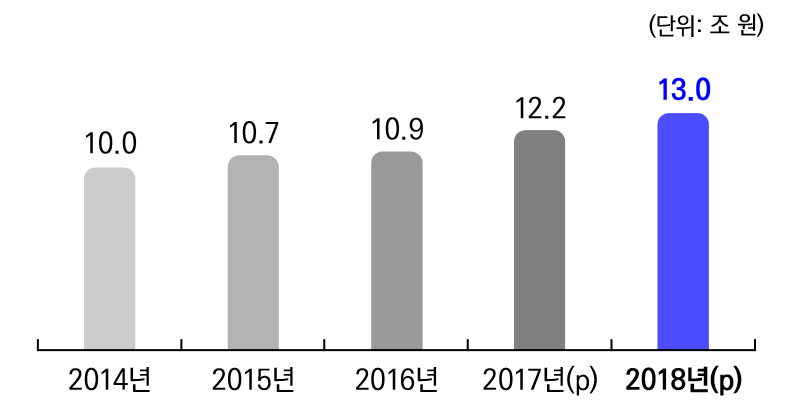
\includegraphics[width=0.7\textwidth]{Pictures/GameMaechul.png}
				\caption{게임 산업 매출액 추이}
			\end{figure}
			
			또한 최근에는 \textbf{E-SPORTS 산업}의 성장으로 인해 \textbf{2020년까지 꾸준히 상승}할 것으로 전망되었으며, \footnote{한국콘텐츠진흥원 대한민국 게임백서 2018 6p} 
			\textbf{VR 기술}의 비약적인 발전과 \textbf{모바일 게임} 시장의 확대로 인하여 앞으로의 발전 가능성이 높은 산업이라 여겨지고 있다.
			
			이러한 게임 산업의 발전으로 인하여 게임 시장의 중요성은 날로 부각되어가고 있는 추세이다. 따라서 \textbf{IT 경영과}에 재학 중인 학생으로서 IT 시장의 신흥 강자로 떠오르고 있는 \textbf{게임 시장}을 분석해보는 것은 4차 산업혁명을 이해하고 대비하는 과정에 있어서 무척이나 도움이 될 것이라 판단하게 되었다.
			
			그중에서도 이번 연구 대상으로 선정된 \textbf{"엔씨소프트"}는 국내에서 오랜 세월 명목을 이어오고 있는 게임 개발사 중 하나이며, 한때 온라인 게임계에 이름을 휘날렸던 \textbf{"아이온"}과 대한민국 게임계에 한 획을 그었다고 평가받는 \textbf{"리니지"} 시리즈를 개발하여 대한민국 게임 시장에 지대한 영향을 미치고 있는 기업이기도 하다. 
			
			이에 대한 통계로, 게임 퍼블리셔를 기준으로 정렬한 \textbf{2019년 상반기 모바일 게임 매출 점유율}을 들 수 있다. 다음은 그것을 도식화 한 것이다
			\footnote{MOBILEINDEX 2019년도 상반기 한국 모바일 게임 시장 총정리 6p}:
			
			
			\begin{figure}[htbp]
				\centering
				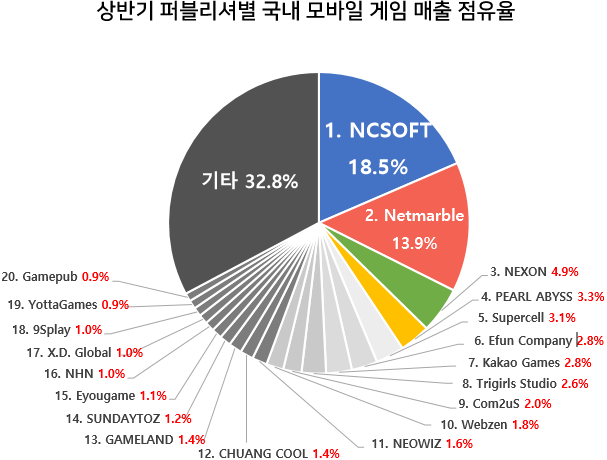
\includegraphics[width=0.8\textwidth]{Pictures/MobileMaechul.png}
				\caption{2019년도 상반기 모바일 게임 매출 점유율 (퍼블리셔별)}
			\end{figure}
			
			이러한 관점에서 엔씨소프트가 \textbf{게임 엔터테인먼트 기업의 표본}으로서 적절한 뿐 만 아니라, 그 경영 전략을 분석하고 연구하기에도 상당히 가치 있는 기업이라 판단하게 되었다.
			
			이에 본 논문에서는 엔씨소프트를 분석함으로서 기업의 비전과 경영 방법이 실적에 미친 영향에 대하여 제시하고자 하며, 궁극적으로는 학과에서 주어진 연구 목적을 달성하기 위하여 결론으로서 \textbf{기업 전망 예측}과 \textbf{발전 방안}을 제시하고자 한다.
					
		\subsection{방법}
			서론을 제외한 본문이 시작되는 2장에서는 심화 분석의 원활한 진행을 위하여 선행 조사를 실시하였다. 선행 조사는 \textbf{기업 개요, 기업 연혁, 기업 비전} 총 3개의 주제로 이루었으며, \textbf{엔씨소프트 공식 홈페이지\footnote{http://kr.ncsoft.com/korean/}}에서 소개하고 있는 자사의 개요, 
			연혁, 비전을 활용하는 것으로 하였다. 
			
			3장에서는 선행 조사를 통하여 수집된 자료들을 기반으로 \textbf{시장, 환경, 경쟁사, 마케팅}의 방면에서 \textbf{통계 자료, SWOT 모델, STP 모델을 활용하여} 분석하였다. 또한 다시 이를 기반으로 경영 실적을 확인하기 위해 \textbf{재무, 주식}에 관하여 분석하였다. 분석용 자료로서는 \textbf{뉴스 보도자료, 신뢰성이 입증된 통계 자료, 엔씨소프트 공식 발표 자료, 네이버 금융 등}을 활용하여 자료의 신뢰성을 확보하였다.
			
			4장에서는 심화 분석 결과를 요약하고, 이를 토대로 하여 \textbf{기업 전망 예측}과 \textbf{발전 방안}을 제시하였다.
			\begin{figure}[htbp]
				\centering
				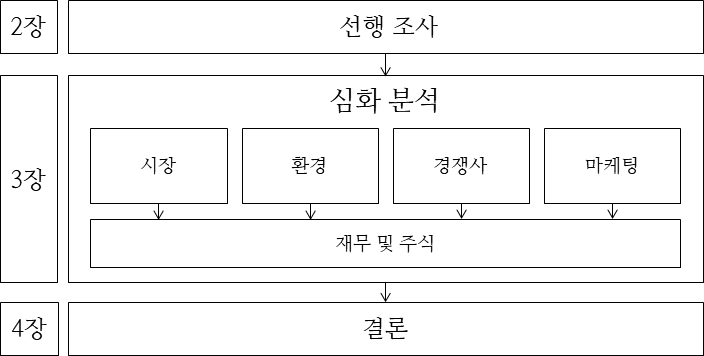
\includegraphics[width=0.8\textwidth]{Pictures/Methods.png}
				\caption{연구 구성}
			\end{figure}
			
	
	\section{선행 조사}
		\subsection{기업 개요}
		\noindent 
		\begin{figure}[htbp]
			\centering
			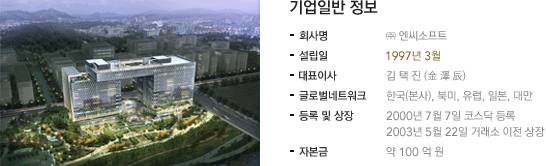
\includegraphics[width=1\textwidth]{Pictures/ncinfo.png}
			\caption{엔씨소프트 일반 정보}
		\end{figure} 
		
		엔씨소프트는 \textbf{온라인, 모바일 게임 개발과 서비스, 디지털 엔터테인먼트 관련 인터넷 사업}을 영위하고 있으며, 1998년 \textbf{리니지}를 시작으로 인터넷 기반 온라인 게임의 대중화를 이끌었다. 또한 종속회사를 통해 소프트웨어 개발과 판매, 프로야구 서비스, 콜센터 서비스 등도 운영 중이며, 이에 그치지 않고 해외 시장을 개척, 아시아, 북미, 유럽 등에 \textbf{글로벌 네트워크}를 확보해 나가고 있다.
		
		엔씨소프트는 본래 창업 당시인 1997년 \~ 1999년까지는 온라인 게임 전문이 아닌 인터넷 기반 기업용 소프트웨어 개발 업체였다. 김택진 CEO가 송재경의 리니지 팀을 인수하여 정식 서비스를 개시한 후, 리니지의 대성공을 발판으로 다른 사업을 정리하고 본격적인 게임 사업에 뛰어들게 되었다.\footnote{[인물열전] '바람의나라' 와 '리니지' 의 아버지, 송재경 - 게임메카}
		
		\textbf{작은 개발사를 인수하여 게임을 서비스}하는 일부 경쟁사들과는 다르게, 대부분의 게임을 \textbf{자사에서 직접 개발하여 서비스}하고 있다. 따라서 비교적 높은 R\&D 능력을 가지고 있으며, 한때 캐주얼 게임에 진출하려 시도한 적이 있었으나 대차게 망하고 온라인 롤플레잉 게임에 주력하고 있다.
		
		\subsection{기업 연혁}
		다음은 엔씨소프트에서 공개하고 있는 연혁 중, 기업의 경영 실적에 영향을 끼쳤으리라 예상되는 부분을 정리한 것이다.
		
		\begin{textbox}	
			\textbf{\textcolor{blue}{1997. 3}} 엔씨소프트 창립			
			\\			
			\textbf{\textcolor{blue}{1998. 9}} 게임  \textbf{리니지} 상용서비스 개시			
			\\			
			\textbf{\textcolor{blue}{2000. 5}} 글로벌 네트워크 구축개시 (해외법인)			
			\\			
			\textbf{\textcolor{blue}{2000. 7}} 해외 서비스 개시 (리니지 대만 서비스 시작)			
			\\			
			\textbf{\textcolor{blue}{2000. 7}} 코스닥 등록(2003년 한국증권거래소로 이전 상장)			
			\\			
			\textbf{\textcolor{blue}{2003. 10}} 게임 \textbf{리니지2} 서비스 개시			
			\\			
			\textbf{\textcolor{blue}{2005. 4}} \textbf{길드워} 상용서비스 개시 (북미 / 유럽 시장)			
			\\			
			\textbf{\textcolor{blue}{2008. 5}} 엔씨소프트 R\&D(Research \& Development) 센터 완공			
			\\			
			\textbf{\textcolor{blue}{2008. 11}} 게임 \textbf{아이온} 서비스 개시			
			\\			
			\textbf{\textcolor{blue}{2009.}} 게임 \textbf{아이온} 글로벌 론칭			
			\\			
			\textbf{\textcolor{blue}{2012. 6}} 게임 \textbf{블레이드 \& 소울} 서비스 개시			
			\\			
			\textbf{\textcolor{blue}{2012. 8}} 게임 \textbf{길드워 2} 상용서비스 개시			
			\\			
			\textbf{\textcolor{blue}{2013. 8}} 판교 R\&D 센터 완공			
			\\			
			\textbf{\textcolor{blue}{2014. 6}} 게임 \textbf{와일드스타} 북미/유럽 상용서비스 개시			
			\\			
			\textbf{\textcolor{blue}{2015. 5}} 북미법인 엔씨웨스트(NC West)의 모바일 스튜디오 설립			
			\\			
			\textbf{\textcolor{blue}{2015. 10}} 게임 \textbf{길드워2: 가시의 심장} 상용서비스 개시			
			\\			
			\textbf{\textcolor{blue}{2016. 1}} 게임 \textbf{블레이드 \& 소울} 북미/유럽 정식 서비스 돌입			
			\\			
			\textbf{\textcolor{blue}{2016. 12}} 게임 \textbf{리니지 레드나이츠} 아시아 12개국 정식 서비스			
			\\
			\textbf{\textcolor{blue}{2017. 6}} 게임 \textbf{리니지 M} 서비스 개시
			\\
			\textbf{\textcolor{blue}{2019. 3}} 게임 \textbf{리니지 리마스터} 출시
			\\
			\textbf{\textcolor{blue}{2019. 11}} 게임 \textbf{리니지2 M} 출시
		\end{textbox}
	
		\subsection{기업 비전 및 사명}
			엔씨소프트는 기업의 주요 비전을 \textbf{Mission, Format, Core Value, Spirit} 총 4가지로 분류하였다. 
			\begin{figure}[htbp]
				\centering
				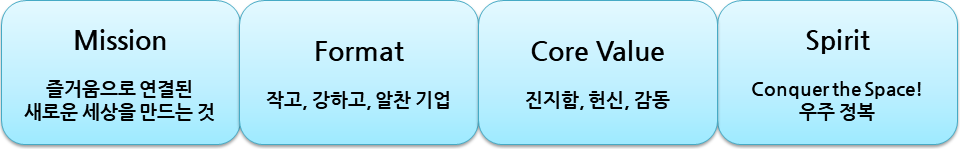
\includegraphics[width=1\textwidth]{Pictures/vision.png}
				\caption{엔씨소프트 기업 비전}
			\end{figure}

			\textbf{Mission}은 엔씨소프트가 이루고자 하는 사명으로, 온라인을 넘어 즐거움으로 연결된 세상을 만들겠다는 결연한 의지를 나타내고 있다.
			
			\textbf{Format}은 \textbf{작고, 강하고, 알찬 기업} 3가지 의미로 나뉜다. 
			\textbf{작다}는 존중을 바탕으로 하나의 팀으로서의 커뮤니케이션이 이루어지는 회사를 의미한다. \textbf{강하다}는 바르게 결정하고 전체가 움직이는 것을 의미한다. \textbf{알차다}는 선택과 집중을 통해 잘하는 일은 누구보다 탁월하게 잘하여 감동을 창조하겠다는 비전을 나타낸다.
			
			\textbf{Core Value}는 기업의 핵심 가치로, \textbf{진지함, 헌신, 감동} 3가지 의미로 나뉜다. \textbf{진지함}은 도덕적, 또는 예술적 가치에 집착하고, 자신이 하는 일에 진지하게 임하겠다는 것을 의미한다. \textbf{헌신}은 엔씨소프트가 스스로 하는 일에 대한 눈부신 열정, 그 열정이 헌신이라 여겨질 정도로 일에 대해 열정을 갖겠다는 것을 의미한다. \textbf{감동}은 사소한 불편을 제거하고자 끊임없이 개선하고, 한 걸음 한 걸음 디테일을 조각해 내어 사람들을 감동시킬 때까지 노력하겠다는 의지를 의미한다.
			
			\textbf{Spirit}은 기업 정신으로, \textbf{Conquer the Space! 우주 정복}이라는 문장으로 표현할 수 있다. 이는 남들이 만들려는 것을 똑같이 개발하려는 것이 아니라, 항상 자신이 꿈꾸는 새로운 세계를 만들어나가야 한다는 엔씨소프트의 정신을 담은 문장이다. 남들이 가지 않은 별을 찾아서 \textbf{'감동'}을 주겠다는 것이 정복의 의미이다.

		\subsubsection{기업 CI}
			\begin{figure}[htbp]
				\centering
				
\includegraphics[width=0.8\textwidth]{Pictures/ci.png}
				\caption{엔씨소프트 기업 CI}
			\end{figure}
			
			로고와 회사 명에 포함되어 있는 'NC'는 창업 당시 Next Company의 의미를 담고 시작했다고 한다. 뜻은 단순히 회사 이름을 정하지 못했던 탓이었다고 한다. 하지만 이내 '영화를 뛰어넘는 게임을 만들자'는 의미에서 'Next Cinema'의 준말로 바뀌게 되었고, 현재에는 다시금 \textbf{'끊임없이 변화하는 회사가 되자'}라는 의미를 담아 \textbf{'Never ending Change'}의 준말로 바뀐 상태이다.
			
			엔씨소프트의 CI는 \textbf{혁신적인 변화와 성장의 의미}를 담고 있으며, 현재에 만족하지 않고 항상 도전하며 끊임없이 창의를 추구하는 엔씨인의 정신을 형상화 한 것이다. N과 C의 연결을 통한 공간과 입체형태는 \textbf{엔씨소프트와 고객이 즐거움으로 연결되는 새로운 세상의 창조}를 의미한다.
			
			또한 엔씨소프트의 기업 컬러로서, 우아함과 완결을 의미하는 \textbf{'골드'}, 견고함과 신뢰를 의미하는 \textbf{'다크블루'}, 순수함과 무한을 의미하는 \textbf{'순백색'}을 하나로 모아 창의적이며 미래지향적인 기업 정체성을 반영하였다.
			
	\section{본론}
		\subsection{시장 분석}
		최근의 게임 시장은 PC 게임 보다는 \textbf{모바일 게임}쪽으로 확대되고 있다고 볼 수 있다. 특히나 \textbf{'롤플레잉'} 장르의 게임이 시장의 주류를 이루게 되었는데, 이는 수요-공급의 법칙에 따라 \textbf{'롤플레잉 장르에 대한 수요'}의 증가라고 해석할 수 있다. 아래의 도표는 그것을 통계화 하여 원형 차트로 나타낸 것이다.
		\footnote{MOBILEINDEX 2019년 상반기 한국 모바일 게임 시장 총정리 5p}
		\footnote{한국콘텐츠진흥원 2018 대한민국 게임백서 5p}:	
			
		\begin{figure}[htbp]
			\centering
			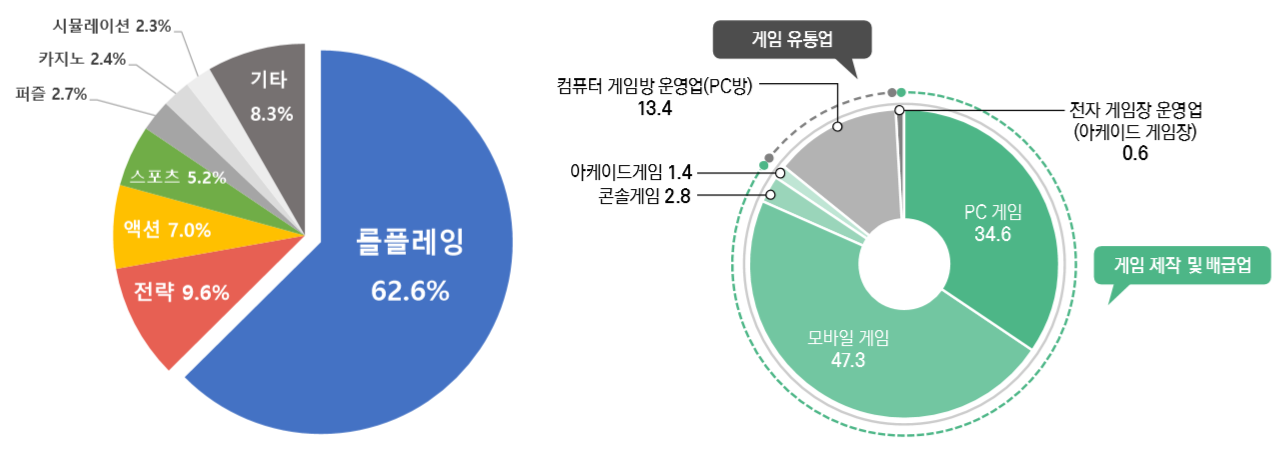
\includegraphics[width=1\textwidth]{Pictures/marketpiechart.png}
			\caption{2019 상반기 장르별 모바일 게임 매출 점유율 현황 및 국내 게임 시장의 분야별 비중}
		\end{figure}
		
		이러한 \textbf{시장 조건}은 올해 10월 출시한 '리니지2 M'과 같이 최근 모바일 게임 시장에 투자하며 거의 MMORPG 게임만 개발하는 \textbf{엔씨소프트에게 매우 유리하다고 볼 수 있다.} 
		
		하지만 이는 양날의 검으로, 추후 '롤플레잉' 게임 보다는 다른 장르의 수요가 증가하여 주류를 이루게 될 시에 이미 한 번 캐주얼 게임으로 대차게 말아먹은 전적을 가진 엔씨소프트는 장세에 대응할 수 있는 방법이 마땅치 않다.
	
		다음은 2019년 상반기 매출 상위 7개 모바일 게임을 정리한 도표이다.  \footnote{MOBILEINDEX 2019년 상반기 한국 모바일 게임 시장 총정리 9p}
		\begin{figure}[htbp]
			\centering
			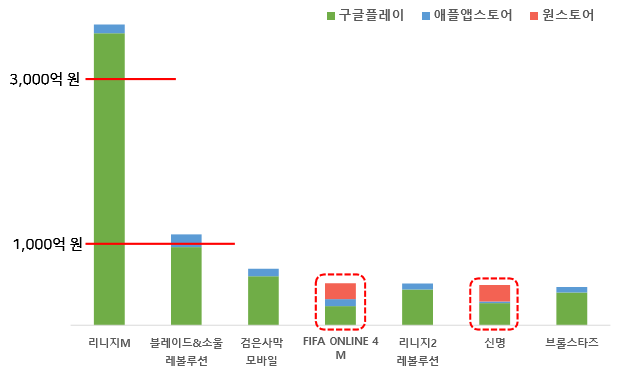
\includegraphics[width=0.8\textwidth]{Pictures/Sangbangi.png}
			\caption{2019년 상반기 매출 TOP7 모바일 게임}
		\end{figure}

		\textbf{상위 매출 모바일 게임 1위}가 엔씨소프트의 \textbf{리니지M}이다. \textbf{리니지M}은 엔씨소프트가 개발과 배급을 모두 담당하였다. 연혁에서 확인할 수 있듯이, 리니지 M은 2017년 출시된 게임으로 올해 뿐 만 아니라, \textbf{출시 이후 2년 연속 매출 1위}를 기록하고 있다.
		\footnote{http://www.thegames.co.kr/news/articleView.html?idxno=212779, '리니지 M' 2년 연속 매출 1위 '맹렬 질주'}
		매출 2위와 매출 3위의 점유율을 합쳐도 리니지M의 점유율에 미치지 못한다. 심지어 매출 2위인 블레이드\&소울 레볼루션의 IP는 본래 엔씨소프트의 것이다.
		
		심지어 작년에는 \textbf{리니지 2 레볼루션}과 
		\textbf{리니지M}이 18년도 하반기 구글플레이 시장 규모를 \textbf{2배 가까이} 늘려놓아 \textbf{한국 구글 플레이 연도별 누적 매출 최초 3조 돌파}라는 실적을 달성할 수 있었다.\footnote{https://www.mk.co.kr/news/it/view/2017/12/821784/, ‘리니지의 힘’ 韓 구글 플레이 사상 최초 누적매출 3조 돌파} 모바일 게임 시장이 대세인 현재, 그것도 모바일 게임 시장에서 가장 큰 영향력을 가지고 있는 구글플레이의 매출을 들었다 놓았다 하는 것을 보면 \textbf{지금 당장의 엔씨소프트 시장 영향력은 가히 어마어마하다고 할 수 있다.}
		
		\subsection{경쟁사 분석}
		경쟁사로는 흔히 게임 업계에서 엔씨소프트와 함께 \textbf{'3N'}이라 불리는 \textbf{넥슨}과 \textbf{넷마블}을 들 수 있다. 안타깝게도 엔씨소프트는 이 중에서도 3위를 차지하고 있다. 
		
		그에 관해서 분석해 보자면, 게임 관련 빅데이터 분석 기관인 'Superdata'는 최근 9월 넥슨 배급의 \textbf{'던전 앤 파이터'}가 \textbf{전세계 PC 게임 매출 1위}를 달성하였다고 발표하였다. 
		
		\begin{figure}[htbp]
			\centering
			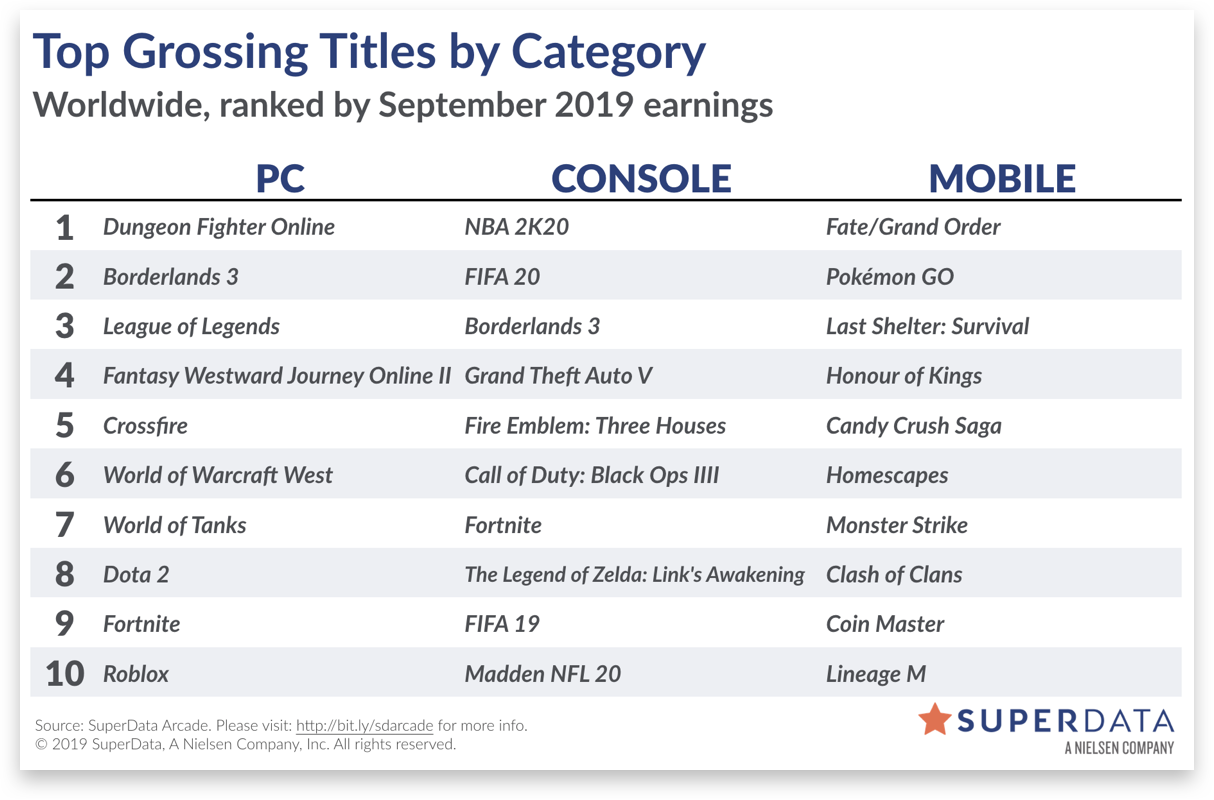
\includegraphics[width=0.9\textwidth]{Pictures/septemberMaechul.png}
			\caption{2019년 9월 카테고리 별 매출 순위}
		\end{figure}
		
		\begin{figure}[htbp]
			\centering
			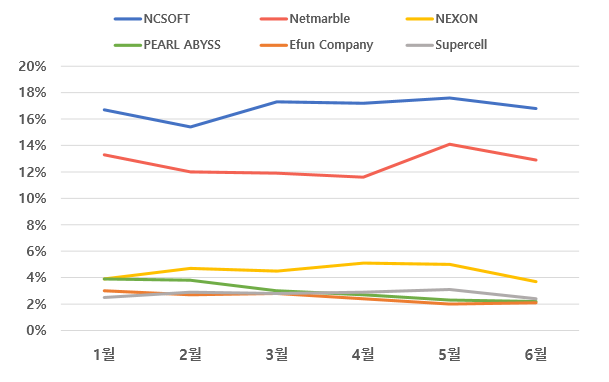
\includegraphics[width=0.9\textwidth]{Pictures/PublisherMaechul.png}
			\caption{2019년 상반기 퍼블리셔별 국내 모바일 게임 매출 점유율}
		\end{figure}
		
		PC 시장에서는 많이 밀린 모습을 보여주고 있지만, '리니지 M' 또한 국내 모바일 게임으로는 유일하게 세계 매출 10위권에 진입함으로서 모바일 시장에서는 강세를 보여주고 있다.
		
		위의 그래프 \footnote{MOBILEINDEX 2019년 상반기 한국 모바일 게임 시장 총정리 6p}는 2019년 상반기 매출 상위 여섯 퍼블리셔의 국내 모바일 게임 매출 점유율을 나타낸 것으로, 엔씨소프트의 그래프가 전 구간에 걸쳐 경쟁사들 보다 높은 곳에 위치한 것을 볼 수 있다. 모바일 게임의 매출이 엔씨소프트 매출 구성의 54\%를 차지하는 상황을 생각해보면 나쁘지 않은 실적이라 생각해볼 수 있다.
		
		또한 '3N' 중 1위를 차지하고 있는 넥슨은 사실상 위에서 기술한 \textbf{'던전 앤 파이터'}에 상당히 의존하고 있는데, 최근에는 업데이트가 중국에서 좋은 반응을 얻지 못하며 지난 2분기 넥슨의 중국 매출액이 2257억원으로 전년 동기 대비 8.2\% 감소했다고 한다. 
		이에 대한 파급으로는 넥슨 일본법인에서 \textbf{시가총액 3조원이 하루만에 증발}했으며, 비록 다시 매출 1위 자리는 확보했어도 국내에서 8월 달 이후로 떨어진 주가는 회복하지 못하고 있는 추세이다.
		\footnote{http://www.donga.com/news/article/all/20190827/97131096/1, 김정주 vs 김택진, 엇갈린 운명?…엔씨 ‘웃고’ 넥슨 ‘울고’}
		
		2위인 넷마블 또한 급성장으로 2017년 엔씨소프트의 자산 총계를 앞질렀지만, 올해 7월에 있었던 \textbf{넥슨 인수}건 무산 이후로 주가가 하락하여 현재까지 쉽게 회복하고 있지 못하는 추세이다. 최근에는 넷마블의 \textbf{웅진 코웨이 인수} 관련 소식으로 주가가 휘청거리고 있다.

		\subsection{환경 분석}
		앞서 한 분석들을 토대로 SWOT 분석 모델을 활용하였다. 결론의 발전 방안 제시안에서 이를 기반으로 SWOT 전략을 수립하기 위함이다.
		
		\begin{figure}[htbp]
			\centering
			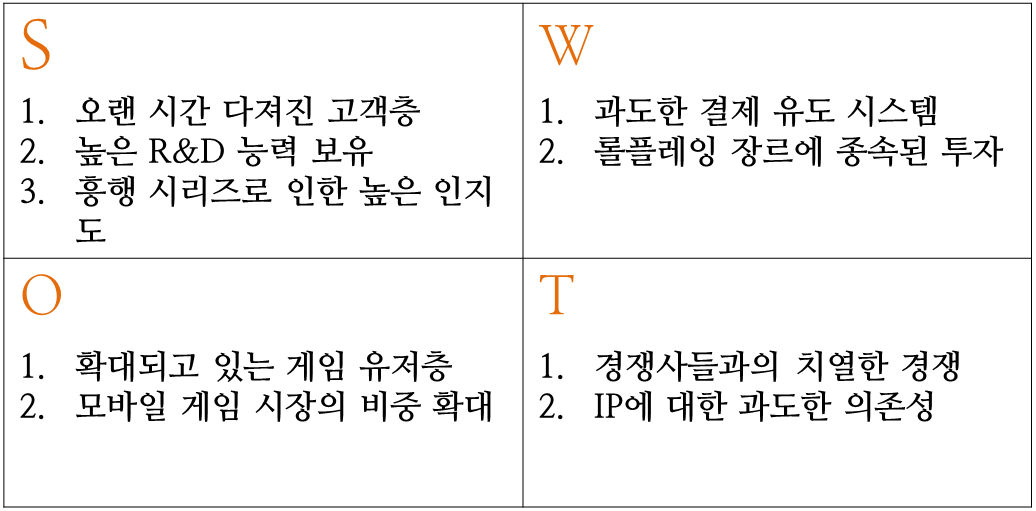
\includegraphics[width=0.9\textwidth]{Pictures/SWOT.png}
			\caption{엔씨소프트 SWOT 분석}
		\end{figure}
	
		\subsection{마케팅 분석}
		엔씨소프트 게임의 이용자 주요 연령대 통계를 기반으로 STP 분석 모델을 사용하였다.
		\begin{figure}[htbp]
			\centering
			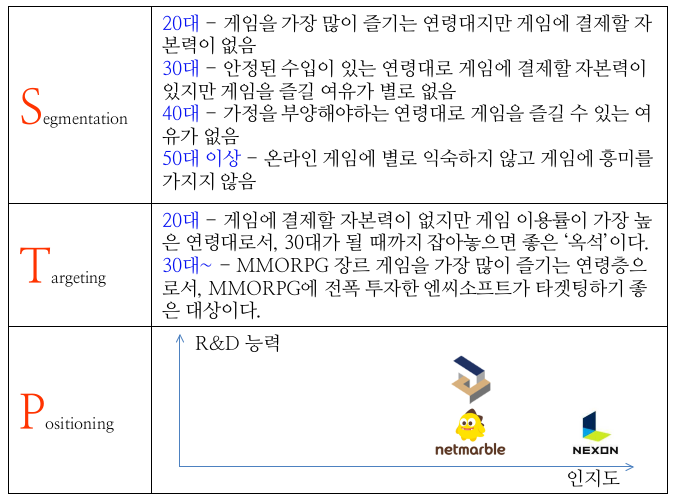
\includegraphics[width=0.9\textwidth]{Pictures/STP.png}
			\caption{엔씨소프트 STP 분석}
		\end{figure}
		
		\subsection{주가 분석}
		엔씨소프트는 2000년 코스닥에 최초 상장이 이루어졌으며, 2003년 코스피로 이전 상장 하였다.. 시가 총액은 \textbf{11조 8,332억 원}으로 코스피 내에서 26위를 차지하고 있다. 
		
		\textbf{전체적으로 살펴보았을 때,} 엔씨소프트의 주가 흐름은 크게 \textbf{3번의 상승}과 \textbf{2번의 하락}으로 이루어진 5단계로 나눌 수 있었다. 이러니 저러니 했지만 결국에는 저번 달에 \textbf{최고가 558,000원}을 달성한 것을 확인할 수 있었다. 이는 최근 '리니지2 M' 출시의 기대 효과로, '리니지 M'의 사례로 전망할 때 근 몇 달 간은 \textbf{주가의 꾸준한 상승이 예상}된다고 할 수 있다.
		
		\pagebreak
		
		\begin{figure}[htbp]
			\centering
			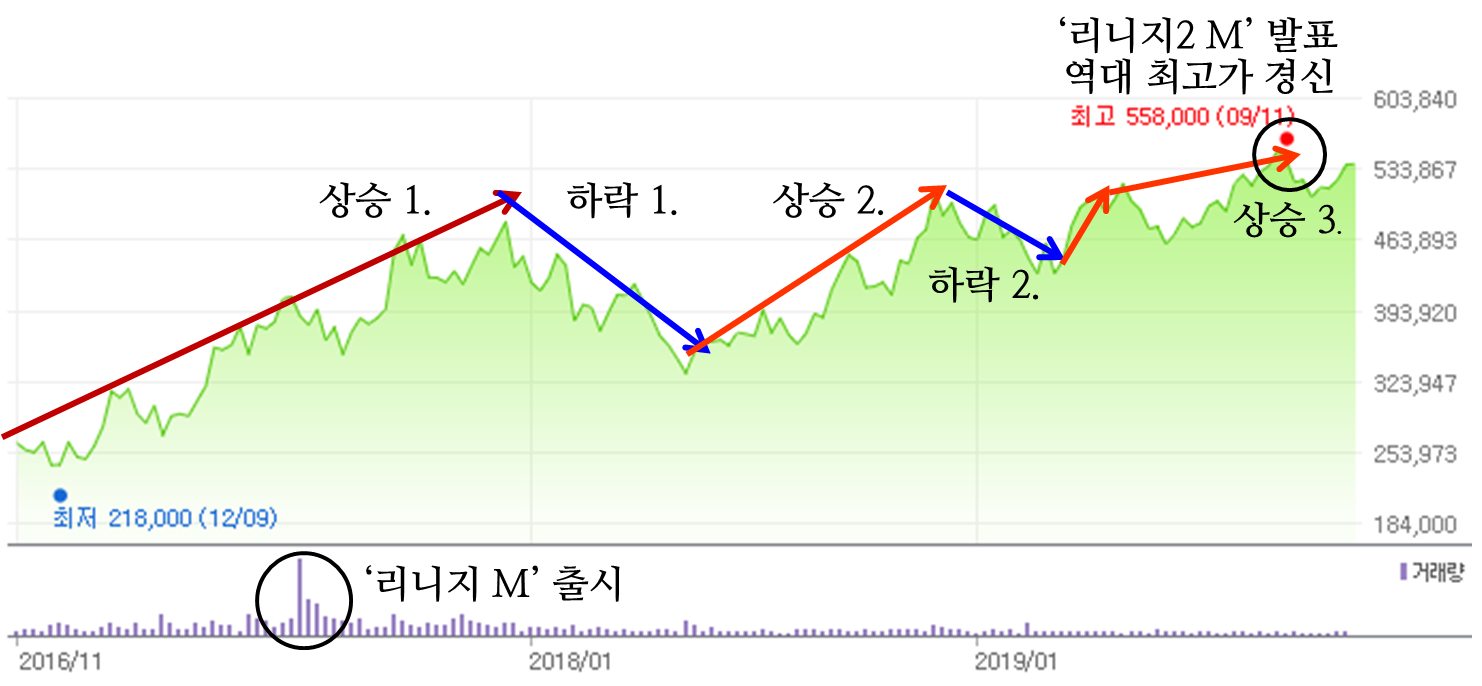
\includegraphics[width=1\textwidth]{Pictures/stock.png}
			\caption{엔씨소프트 주가 (2016/11 - 2019/11)}
		\end{figure}
		
		\textbf{상승 1}은 2016.11 - 2017.12 구간이다. \textbf{초반 상승세}의 요인으로는 \textbf{리니지 RK}의 출시를 통한 모바일 게임 시장 안착과 \textbf{리니지 2 : 레볼루션}에서 넷마블과 맺은 매출 10\% IP 수익 계약을 통한 실적 개선 기대를 꼽을 수 있다. 이 흐름을 이어 \textbf{중-후반 상승세}는 2017년 \textbf{리니지 M}의 기대 효과 및 출시 후 흥행으로 인한 \textbf{역대급 거래량 폭발}과 동시에 \textbf{코스닥의 상승세}로 인한 외국인의 코스피 매도 보류까지 겹쳐진 결과이다. 전체적으로 차트가 꽤 긴 시간 우상향의 지지선과 저항선을 따라갔지만, 18년 1월에 들어선 후 지지선을 하향 돌파하고 주가가 하락세를 보이기 시작하였다. 
		
		\textbf{하락 1}은 2018.1 - 2018.5 구간이다. \textbf{전체적인 하락세}의 요인으로는 미국발 악재에 트리플 약세로 인한 \textbf{외국인 자금 이탈}, 한중 갈등으로 인한 중국 소비 감소와 기타 사유로 인한 \textbf{실적 부진}, \textbf{상반기 신작의 부재}를 이유로 들 수 있었다. 하락세가 길지는 않았지만, \textbf{상승 1}에서 달성했던 주가가 \textbf{반토막}났다. 이후 곧 2018.5 경에 저항선을 돌파하며 다시 상승세를 잇기 시작하였다.
		
		\textbf{상승 2}는 2018.6 - 2018.12 구간이다. \textbf{전체적인 상승세}의 요인으로는 리니지 M 업데이트로 인한 \textbf{실적 향상}과 엔씨소프트의 신작 발표로 인한 \textbf{기대효과}를 꼽을 수 있었다. 마찬가지 상승세가 길지는 않았지만, \textbf{하락 1}에서 반토막 났던 주가가 다시 원 상태를 되찾았다.
		
		\textbf{하락 2}는 2018.12 - 2019.2 구간인데, 그냥 단순하게 \textbf{게임주의 단체 실적 부진}으로 인한 하락세였다.
		
		\textbf{상승 3}은 2019.2 - 2019.11 구간이다. \textbf{초반 상승세}의 요인으로는 \textbf{리니지 리마스터 출시}, \textbf{1분기 실적 시장 기대 부합}, \textbf{리니지 M 일본 진출}을 꼽을 수 있었다. \textbf{중-후반 상승세}의 요인으로는 초반 상승세 요인에 따른 \textbf{실적 향상}, 엔씨소프트 R\&D의 AI 기술에 대한 \textbf{기대효과}, \textbf{리니지2 M 출시 기대효과}를 꼽을 수 있었다. 그리고 마침내 엔씨소프트는 \textbf{역대 최고가}를 경신한다.
		
		\subsection{재무 분석}
		엔씨소프트의 재무상태표를 기반으로 작성한 \textbf{자산 및 부채 변동 그래프}이다.
		
		\begin{figure}[htbp]
			\centering
			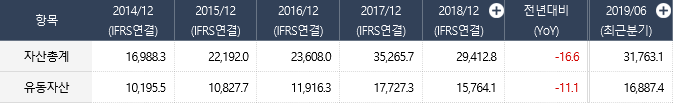
\includegraphics[width=1\textwidth]{Pictures/zaemustate2.png}
		\end{figure}
		
		\begin{figure}[htbp]
			\centering
			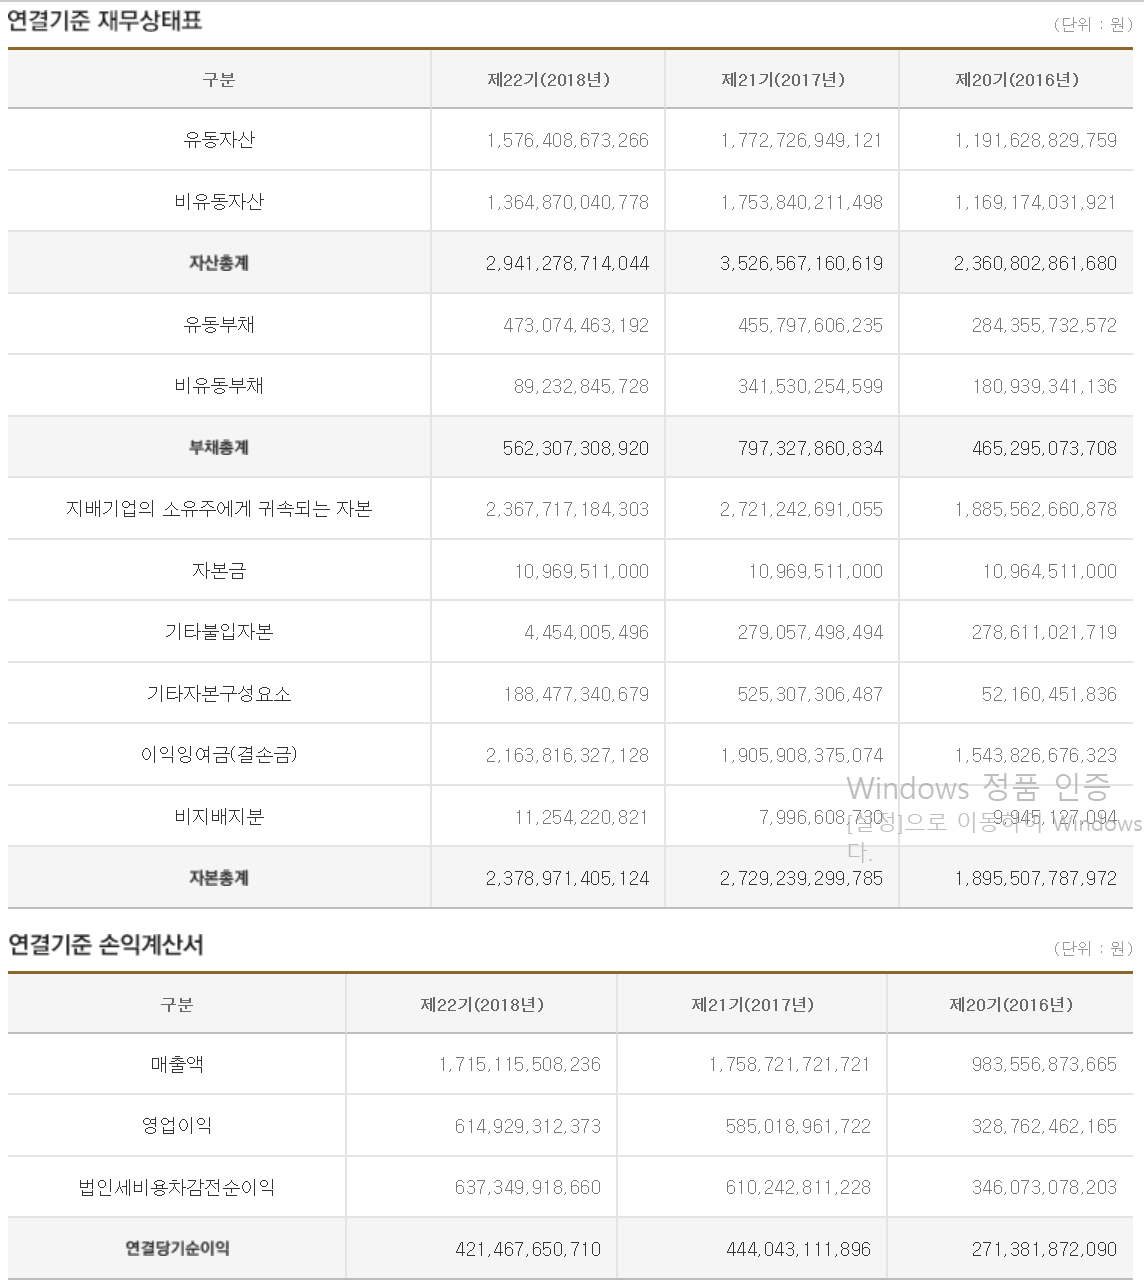
\includegraphics[width=0.8\textwidth]{Pictures/zaemustate.png}
			\caption{엔씨소프트 재무상태표 자산 항목과 자산 및 부채 변동 그래프}
		\end{figure}
		
		엔씨소프트의 총 자산은 전체적으로 보았을 때 전반적으로 성장하는 추세이나, 2018년 잠시 주춤하였다가 다시 회복하는 모습을 보여주고 있다.
		
	\section{결론}
	
	\subsection{전망 예측}
	
	\subsection{발전 방안}
	\begin{figure}[htbp]
		\centering
		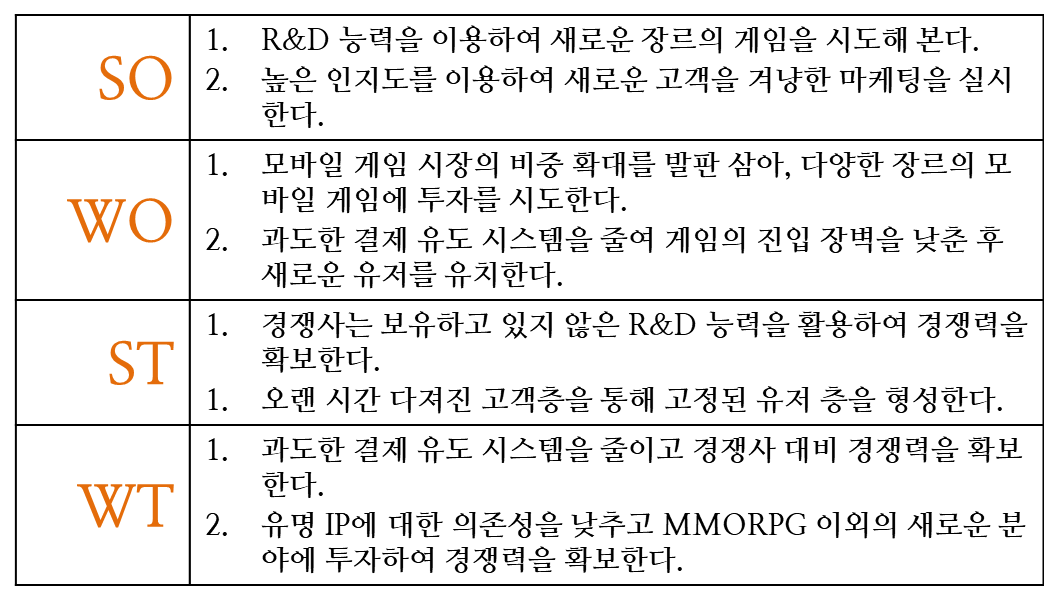
\includegraphics[width=1\textwidth]{Pictures/SWOT2.png}
		\caption{엔씨소프트 SWOT 분석을 기반으로 한 SWOT 전략}
	\end{figure}
	
	\pagebreak
	\section{레퍼런스}
		\noindent
		\textbf{콘텐츠산업 2018년 결산 및 2019년 전망 보고서}
		\\
		http://www.kocca.kr/cop/bbs/view/B0000147/1837529.do
		\\
		\\
		\textbf{한국콘텐츠진흥원 대한민국 게임백서 2018}
		\\
		http://www.kocca.kr/cop/bbs/view/B0000146/1837580.do
		\\
		\\
		\textbf{MOBILEINDEX 2019년도 상반기 한국 모바일 게임 시장 총정리}
		\\
		https://www.mobileindex.com/report/mi\_report\_game\_first\_half\_2019.pdf
		\\
		\\
		\textbf{엔씨소프트 공식 홈페이지} 
		\\
		http://kr.ncsoft.com/korean/
		\\
		\\
		\textbf{인물열전 - '바람의나라' 와 '리니지' 의 아버지, 송재경}
		\\
		https://www.gamemeca.com/view.php?gid=301232
		\\
		\\
		\textbf{'리니지 M' 2년 연속 매출 1위 '맹렬 질주'}
		\\
		http://www.thegames.co.kr/news/articleView.html?idxno=212779
		\\
		\\
		\textbf{‘리니지의 힘’ 韓 구글 플레이 사상 최초 누적매출 3조 돌파}
		\\ 
		https://www.mk.co.kr/news/it/view/2017/12/821784/
		\\
		\\
		\textbf{김정주 vs 김택진, 엇갈린 운명?…엔씨 ‘웃고’ 넥슨 ‘울고’}
		\\
		http://www.donga.com/news/article/all/20190827/97131096/1
		\\
		\\
		\textbf{서울경제}
		\\
		https://m.sedaily.com/Stock/036570
		\\
		\\
		\textbf{네이버 금융}
		\\
		https://finance.naver.com/item/main.nhn?code=036570
		\\
		\\
		\textbf{Company Wise 엔씨소프트 분석}
		\\
		https://comp.wisereport.co.kr/company/c1010001.aspx?cn=\&cmp\_cd=036570
	

\end{document}